\chapter{Các giải pháp, đóng góp nổi bật và minh họa các
chức năng của hệ thống}
\section{Vấn đề lựa chọn công nghệ}
\subsection{Công nghệ front-end}
Công nghệ front-end hiện nay phát triển rất nhanh và rộng.
Có rất nhiều các phương pháp tiếp cận lập trình front-end, đi kèm
là rất nhiều các thư viện, ngôn ngữ, framework,
công cụ hỗ trợ. Mỗi một công nghệ mới ra đời đều đáp ứng
tốt nhu cầu thị trường tại thời điểm đó và
khắc phục được những nhược điểm của các công nghệ cũ.
Ví dụ trước đây một lập trình viên front-end chỉ cần
biết về HTML, CSS mà JavaScript để xây dựng một trang web
thỏa mãn nhu cầu người dùng. Tuy nhiên theo thời gian, nhu cầu
người dùng về tính tương tác của trang web ngày càng cao dẫn
tới sự phát triển mạnh mẽ của ngôn ngữ JavaScript và các thư viện,
framework xây dựng từ đó như thư viện JQuery, EmberJS hay các
thư viện / framework nổi tiếng được dùng phổ biến hiện nay là
ReactJS, Angular, VueJS.

Dựa theo xu thế công nghệ hiện nay, chúng tôi chọn ReactJS – Redux để
xây dựng phần giao diện khi mà thư viện này có một cộng đồng lớn
và được Facebook phát triển. React-Router để định tuyến, xây dựng
Single Page Application, i18next để triển khai đa ngôn ngữ,
Redux-Saga để xử lý middleware,
gửi request và nhận api từ back-end server. 

\subsection{Công nghệ back-end}
Về phần back-end, ban đầu chúng tôi chọn Java Spring để xây dựng.
Java Spring cũng là một framework mạnh mẽ để xây dựng webserver.
Tuy nhiên, Java Spring phù hợp với xây dựng các ứng dụng web
monolithic (đơn khối) hơn là xây dựng theo mô hình microservices
đang trở thành xu hướng trong thời gian hiện nay. Một
hệ thống kiến trúc theo microservices thông thường sẽ
bao gồm nhiều các service nhỏ nhưng số lượng nhiều thì Java
Spring không phù hợp với những service đó do yêu cầu về tài
nguyên của ứng dụng Java là khá lớn. Vì vậy chúng tôi chọn
Go để xây dựng lại back-end server. Về cơ bản thì Go rất
phù hợp cho việc xây dựng các service trong microservices
do yêu cầu về tài nguyên nhỏ, ngoài ra Go còn hỗ trợ tốt xử
lý đa luồng với Goroutine và Chanel đã trình bày ở phần
công nghệ back-end nên
sẽ có thể tăng số request phục vụ tại cùng một thời điểm của hệ thống.

\subsection{Công nghệ Full Text Search}
Như đã đề cập ở phần công nghệ, trong đồ án này chúng tôi sử
dụng tính năng Full Text Search đã có trên PostgreSQL kết hợp
với sử dụng Index cho các câu truy vấn tìm kiếm người dùng,
khách hàng, tài khoản, tên sản phẩm, \ldots Ban đầu chúng tôi
chọn ElasticSearch cho tính năng này, tuy nhiên để sử dụng
ElasticSearch thì dữ liệu trong PostgreSQL phải được sao lưu
sang ElasticSearch. Để thực hiện việc sao lưu này có thể thực
hiện trên code của web server hoặc sử dụng hệ thống
Change Data Capture như Debezium.

Nếu thực hiện trên code thì không đảm bảo được dữ liệu
ở PostgreSQL và trên ElasticSearch là giống nhau. Đồng thời
sẽ làm code của web server trở nên phực tạp hơn do vừa phải quan
tâm đến dữ liệu của PostgreSQL vừa cả dữ liệu trên ElasticSearch.

Nếu sử dụng hệ thống Change Data Capture như Debezium
thì sẽ giải quyết được hai vấn đề trên, tuy nhiên lại làm hệ thống
phức tạp lên rất nhiều vì phải triển khai cả Kafka làm
kênh trung gian truyền dữ liệu từ PostgreSQL sang ElasticSearch.
Việc sử dụng một công nghệ phức tạp như vậy vượt quá giới
hạn thời gian cho đồ án này. Vì vậy chúng tôi sử dụng cách đơn giản
hơn là tính năng Full Text Search tích hợp sẵn trong PostgreSQL,
khi đó sẽ không phải xét đến vấn đề sao
lưu và tính nhất quán của dữ liệu.

\section{Chức năng phân quyền động}
Phân quyền là tính năng không thể thiếu được trong các trang mang
tính chất quản trị, mỗi người cần phải được giới hạn trong truy cập.
Ví dụ không thể để một nhân viên bán hàng sử dụng được tính năng
quản lý sản phẩm hay giá sản phẩm. Do đó dựa trên các tính năng
đã phân tích như quản lý phân quyền, quản lý sản phẩm, quản lý tài khoản,
quản lý kho, quản lý tuyến bán hàng, … chúng tôi phân chia người dùng
hệ thống vào các security\_group, mỗi security\_group lại có một tập
quyền (permissions). Hệ thống sẽ dựa vào các permission mà người
dùng có để xác định xem họ có thể truy
cập được vào tính năng đó hay không.

\begin{table}[H]
\centering
\begin{tabular}{| m{5cm} | m{11cm} |}
\hline
\textbf{security\_group} & \textbf{security\_permission} \\
\hline
ADMIN &
VIEW\_EDIT\_PARTY, VIEW\_EDIT\_USER\_LOGIN,
VIEW\_EDIT\_SECURITY\_GROUP,
VIEW\_EDIT\_SECURITY\_PERMISSION \\
\hline
PRODUCT\_MANAGER &
VIEW\_EDIT\_PRODUCT \\
\hline
SALES\_MANAGER & 
VIEW\_EDIT\_ORDER \\
\hline
FACILITY\_MANAGER & 
VIEW\_EDIT\_FACILITY \\
\hline
INVENTORY\_MANAGER & 
IMPORT \\
\hline
EXPORT\_MANAGER &
EXPORT \\
\hline
SALESMAN\_MANAGER &
VIEW\_EDIT\_SALESMAN \\
\hline
SALESMAN &
SALESMAN\_CHECKIN \\
\hline
\end{tabular}
\caption{Security\_group và permission tương ứng}
\end{table}

Khi một người dùng được thêm vào hệ thống, họ sẽ được cấp một
user\_login (hiểu như là username), giả sử người này là quản lý
sản phẩm thì sẽ được cấp một quyền VIEW\_EDIT\_PRODUCT, nếu người này
có khả năng quản lý rộng hơn làm được cả nhập kho thì sẽ cấp thêm
quyền IMPORT, … Đường dẫn (url) sẽ được gán theo permission để
kiểm soát truy nhập. Ví dụ PRODUCT\_MANAGER muốn xem danh sách các
sản phẩm thì phải truy cập url có dạng …/view-product,
url này chỉ được truy cập khi có quyền VIEW\_EDIT\_PRODUCT.

% \section{Chức năng phân cụm cửa hàng}
% Đây là một tính năng hoàn toàn mới, theo
% tìm hiểu và khảo sát của chúng tôi
% thì chưa có trên các phần mềm quản lý phân phối hiện nay. Xuất phát
% từ ý tưởng các nhân viên bán hàng hằng ngày phải thăm các cửa hàng bán
% lẻ. Vậy làm thế nào có thể tối ưu được quãng đường di chuyển của nhân
% viên, để họ có thể di chuyển một cách dễ dàng nhất. Và chúng tôi đã đưa
% ra tính năng này, với mục đích là đưa ra gợi ý về các cụm
% cửa hàng gần nhau, giúp người quản lý tuyến bán hàng chọn ra các
% tuyến bán hàng phù hợp.

% Sử dụng thuật toán phân cụm K-Means với đầu vào là N cửa
% hàng bán lẻ trong hệ thống, và K cụm (do người quản lý tuyến
% chỉ định). Đầu ra của thuật toán là K cụm, trong đó là vị trí
% các cửa hàng gần nhau. Tuy nhiên khoảng cách sử dụng không phải là
% khoảng cách Euclidean, mà là khoảng cách Haversine – công thức
% tính khoảng cách giữa hai điểm trên tọa độ thực tế
% (dựa trên kinh độ và vĩ độ).

% Công thức Haversine tính khoảng cách giữa 2 
% điểm $(x_1, y_1)$, $(x_2, y_2)$ trong không gian sử
% dụng kinh độ và vĩ độ:
% \begin{align*}
% &\Delta x = x_1 - x_2 \\
% &\Delta y = y_1 - y_2 \\
% &a = \sin^2 \left( \frac{\Delta x}{2} \right)
%     + \cos \left( x_1 \right) \times \cos \left( x_2 \right) 
%     \times \sin^2 \left( \frac{\Delta y}{2} \right)
%     \\
% &c = 2 \times \arcsin \left( \sqrt{a} \right ) \\
% &d = R \times c
% \end{align*}
% Trong đó: $x_1$, $x_2$ là kinh độ, $y_1$ $y_2$ là vĩ độ, tính bằng radian.
% R là bán kính trái đất (xấp xỉ $6,371$ km). $d$ là khoảng cách cần tìm.

\section{Minh họa các chức năng của hệ thống}
\begin{figure}[H]
\centering
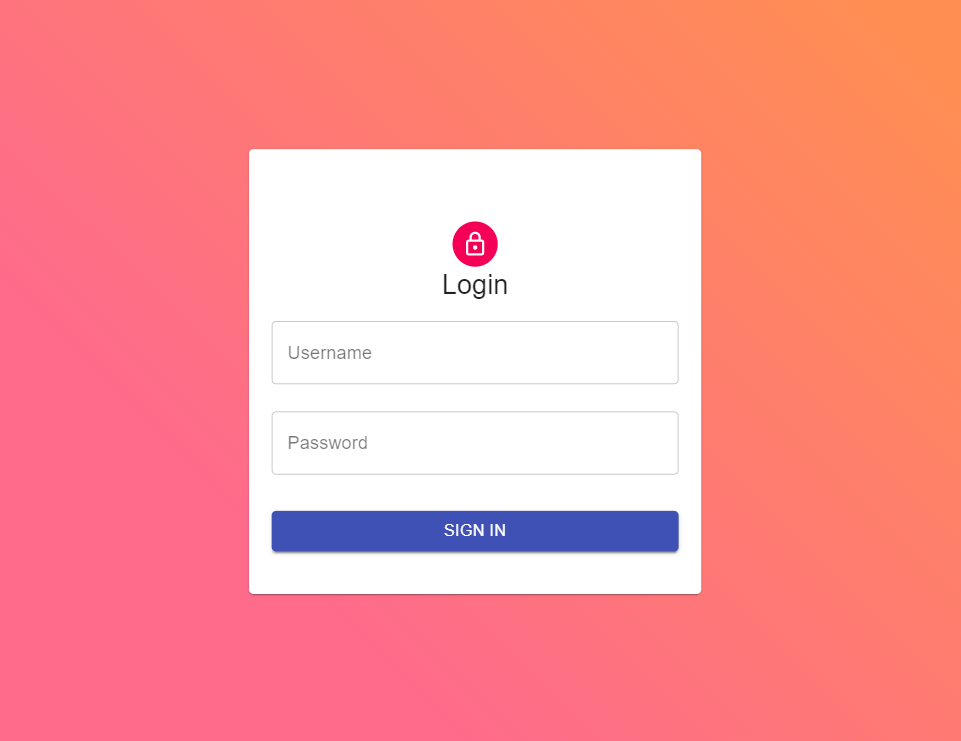
\includegraphics[width=12cm]{images/demo/login.png}
\caption{Chức năng đăng nhập}
\end{figure}

\begin{figure}[H]
\centering
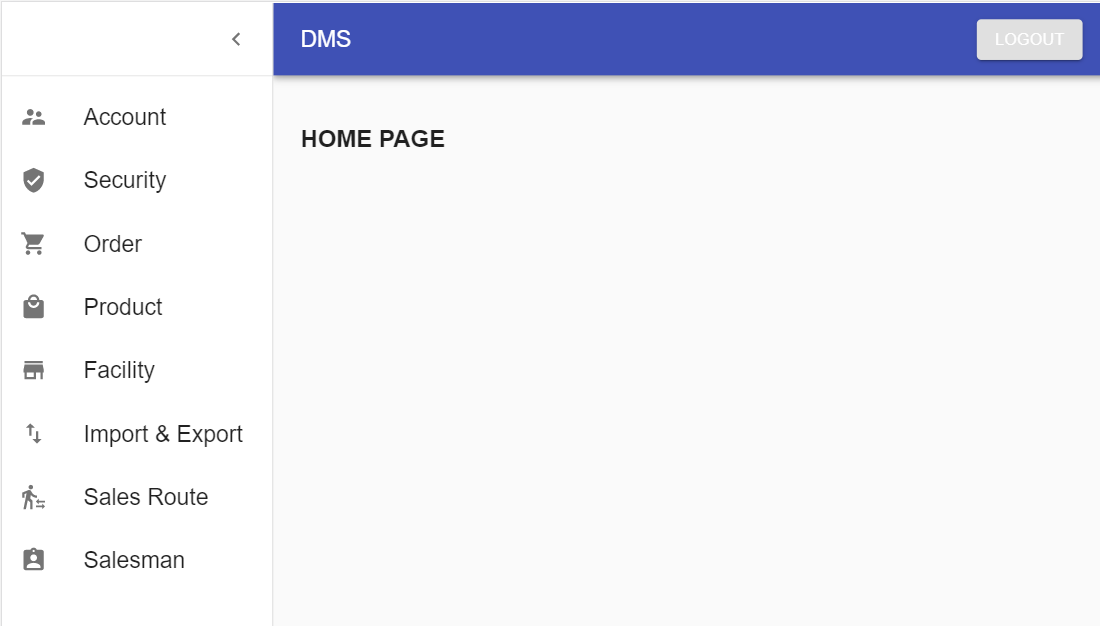
\includegraphics[width=15cm]{images/demo/home-page.png}
\caption{Giao diện trang chủ hệ thống}
\end{figure}

\begin{figure}[H]
\centering
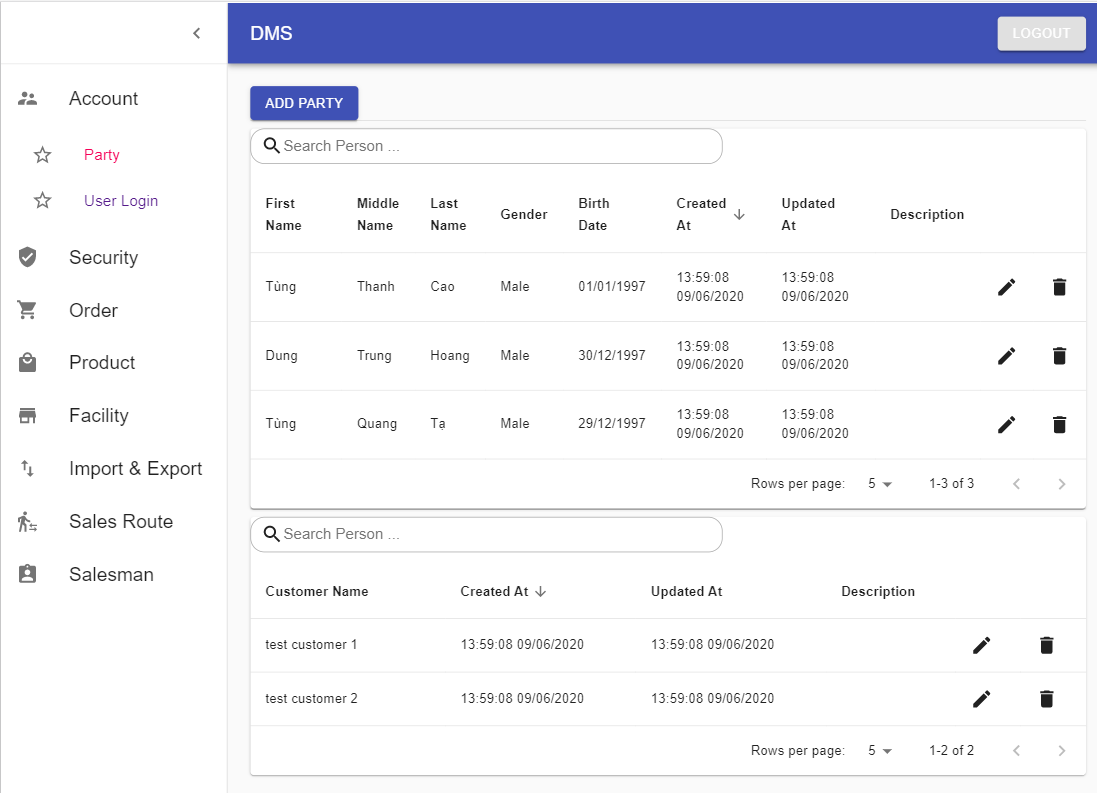
\includegraphics[width=15cm]{images/demo/party-manage.png}
\caption{Quản lý người dùng}
\end{figure}

\begin{figure}[H]
\centering
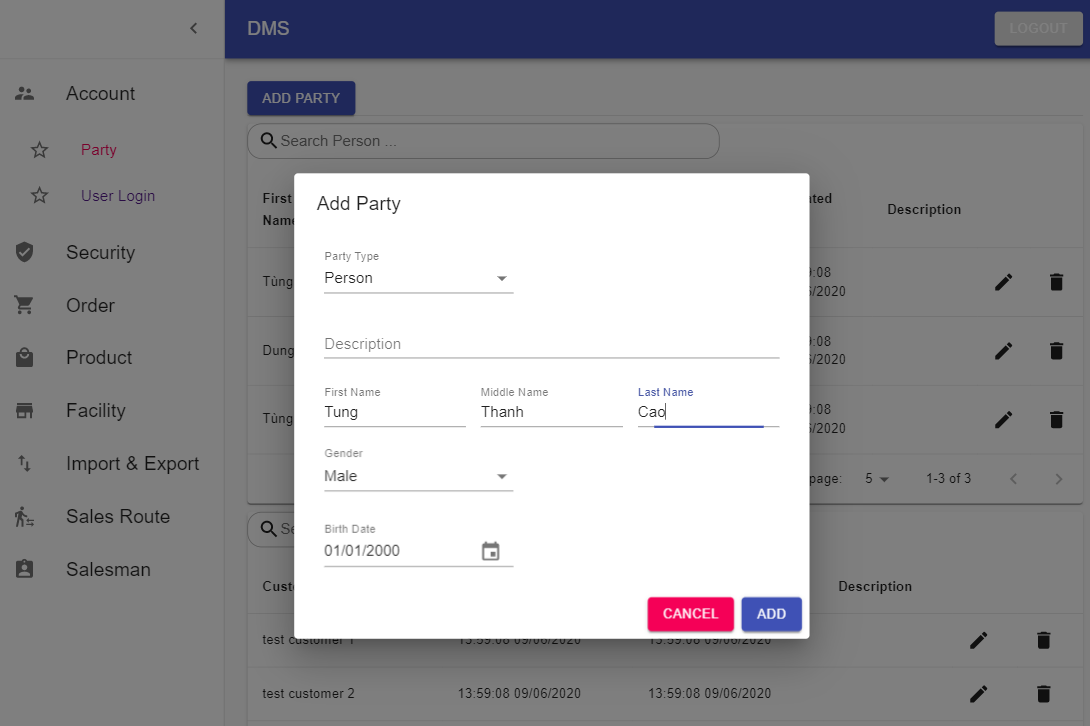
\includegraphics[width=15cm]{images/demo/add-party.png}
\caption{Thêm người dùng / khách hàng}
\end{figure}

\begin{figure}[H]
\centering
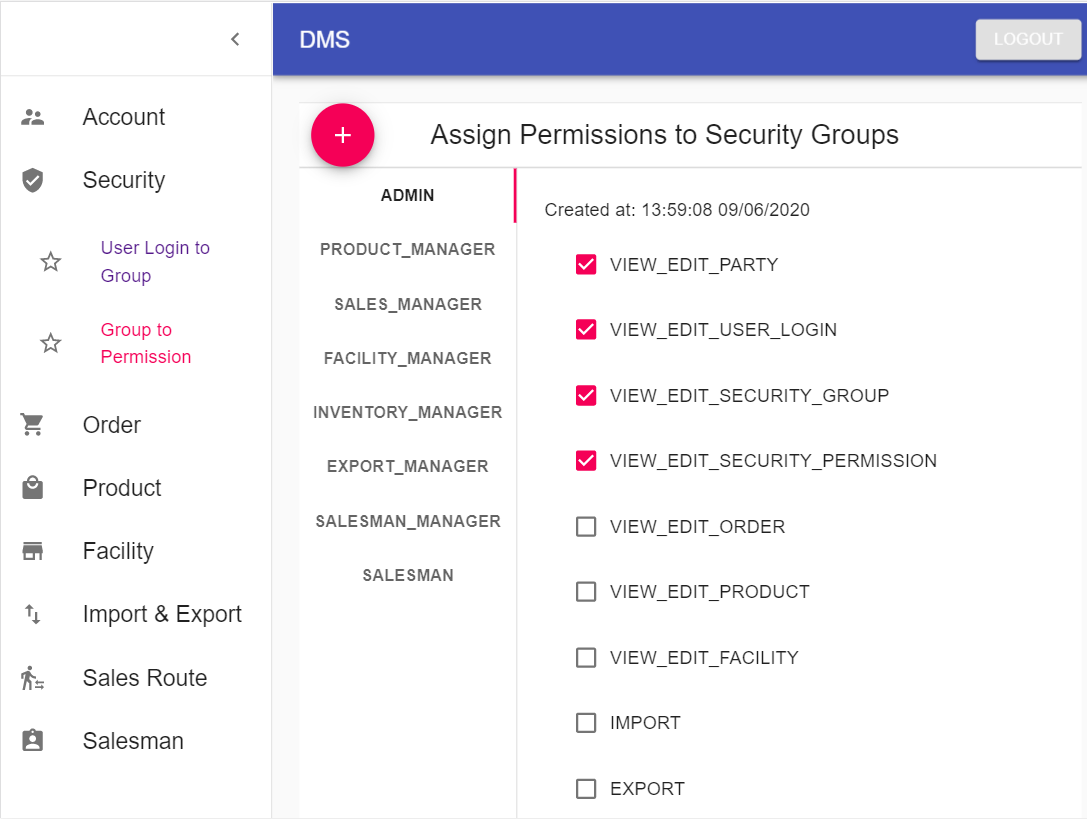
\includegraphics[width=15cm]{images/demo/group-to-permission.png}
\caption{Quản lý các nhóm quyền}
\end{figure}

\begin{figure}[H]
\centering
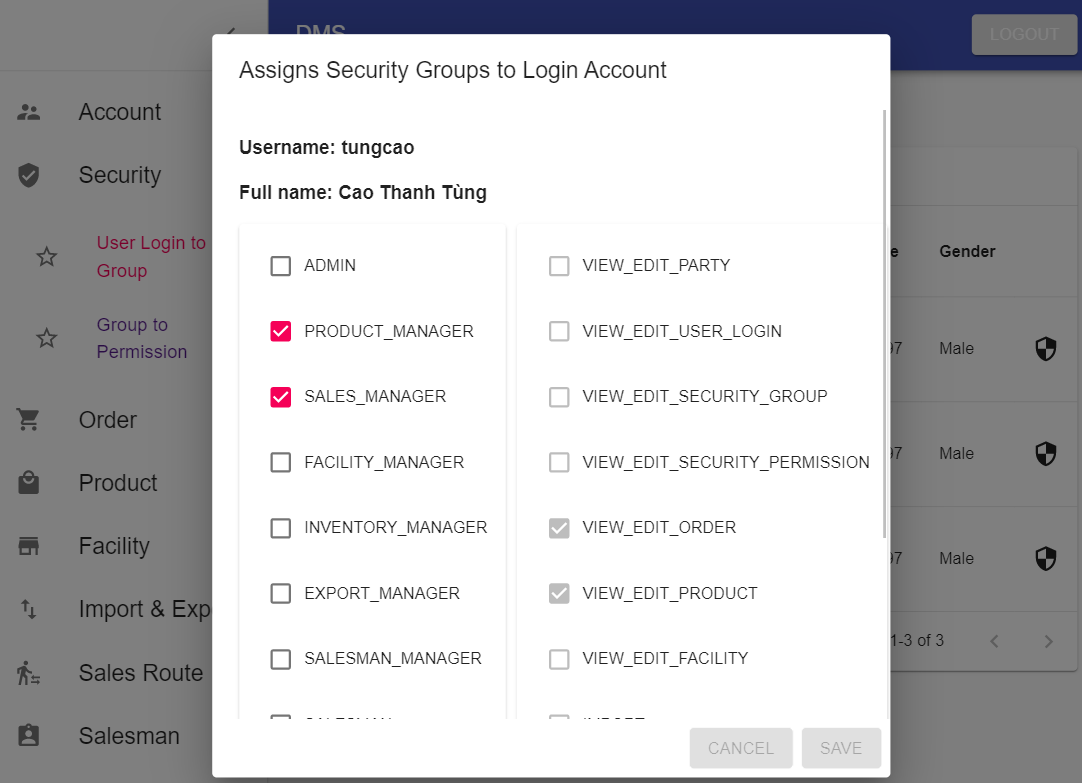
\includegraphics[width=15cm]{images/demo/user-login-to-group.png}
\caption{Gán quyền cho tài khoản người dùng}
\end{figure}

\begin{figure}[H]
\centering
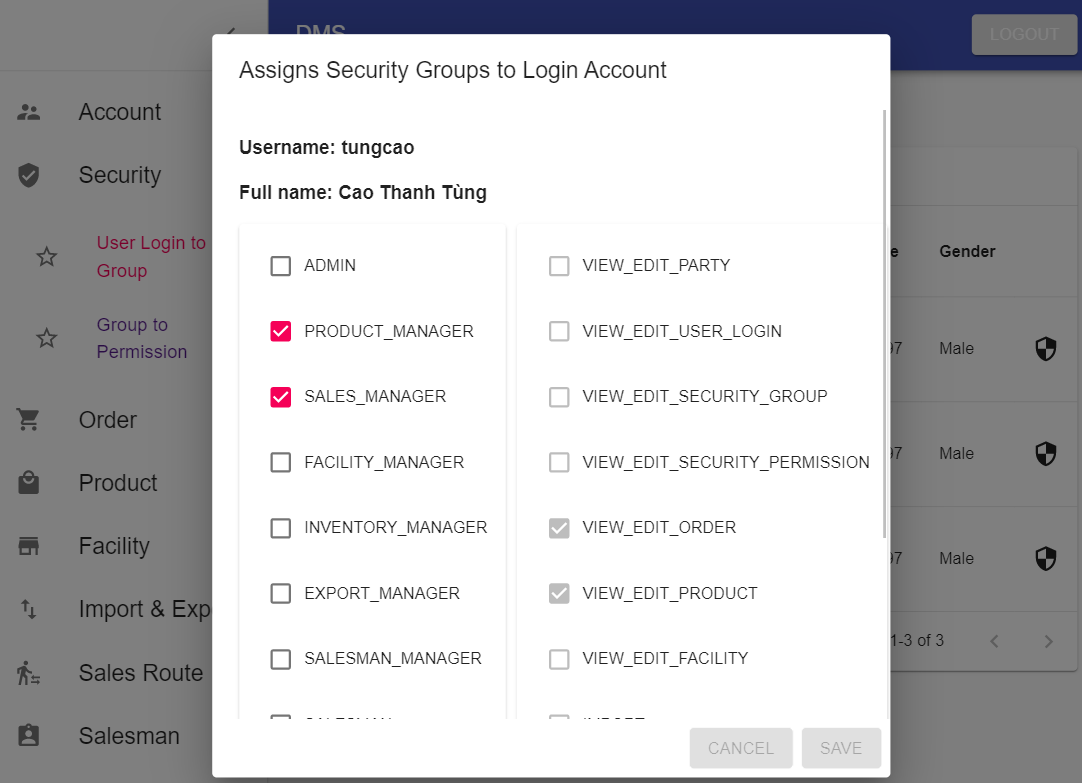
\includegraphics[width=15cm]{images/demo/user-login-to-group.png}
\caption{Gán quyền cho tài khoản người dùng}
\end{figure}

\begin{figure}[H]
\centering
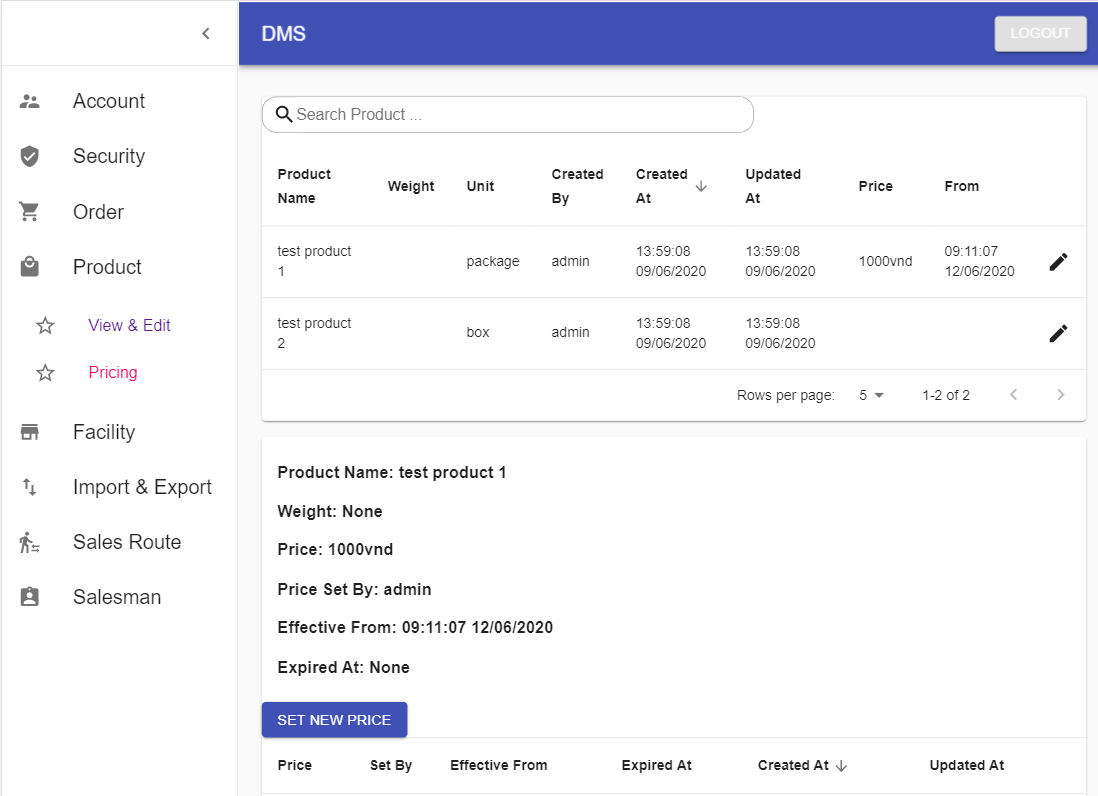
\includegraphics[width=15cm]{images/demo/product-price.png}
\caption{Quản lý giá của các sản phẩm}
\end{figure}

Tạo đơn hàng mới phải qua các bước như chọn khách hàng
(để giao hàng đến), chọn kho chứa hàng hóa, chọn hàng
hóa, nhập địa chỉ (nếu có hoặc chọn kho của cửa hàng).
\begin{figure}[H]
\centering
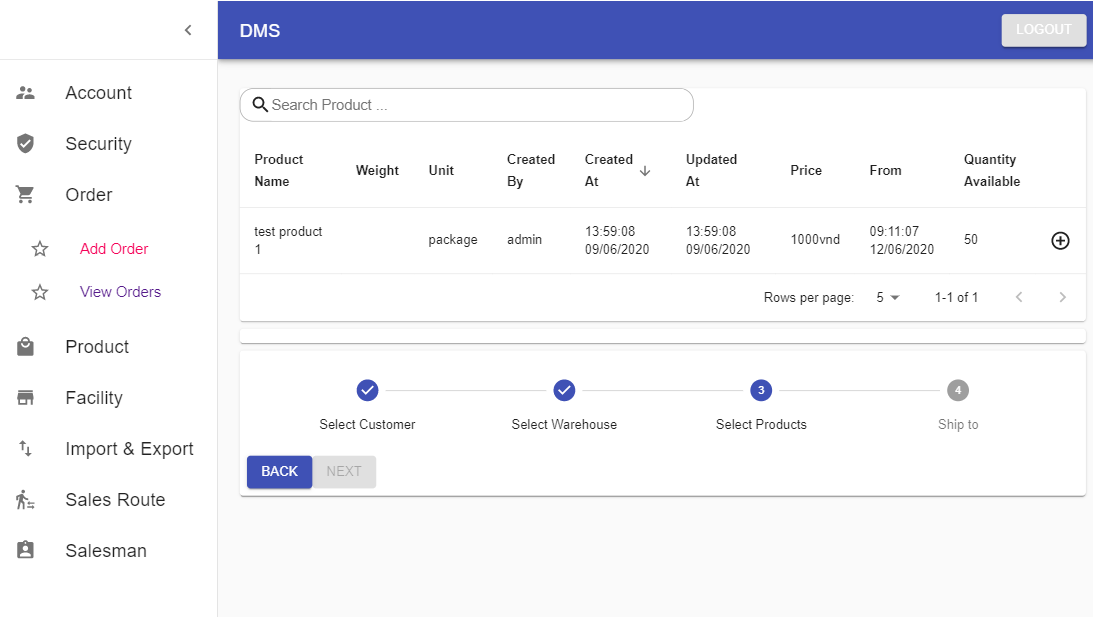
\includegraphics[width=15cm]{images/demo/add-order.png}
\caption{Tạo đơn hàng}
\end{figure}

\begin{figure}[H]
\centering
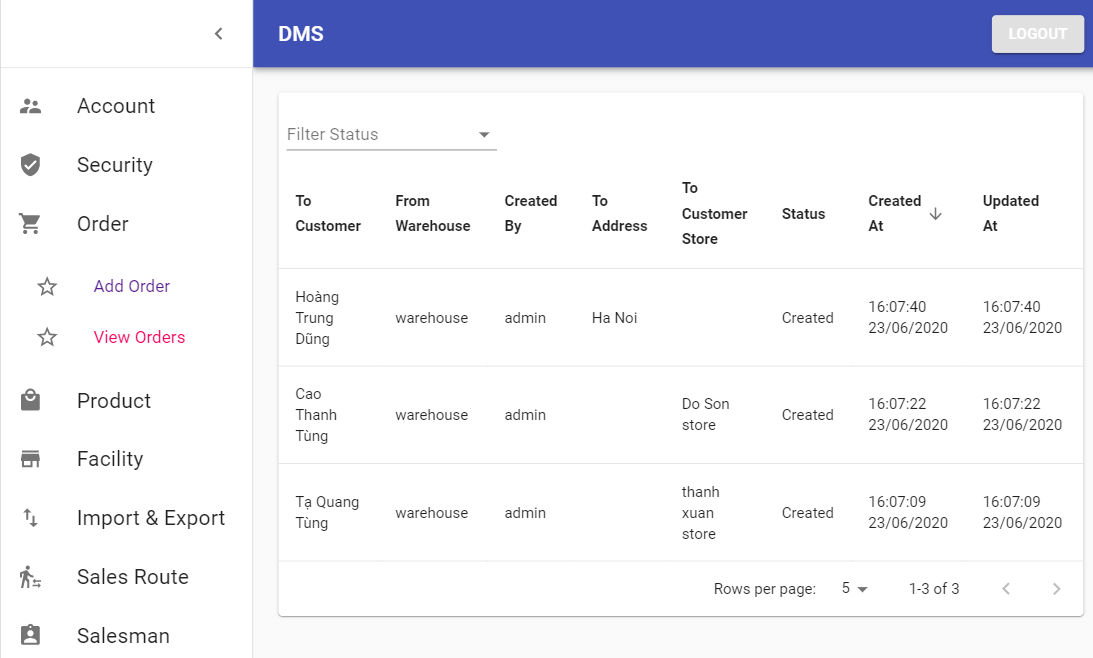
\includegraphics[width=15cm]{images/demo/view-orders.png}
\caption{Hiển thị đơn hàng}
\end{figure}

\begin{figure}[H]
\centering
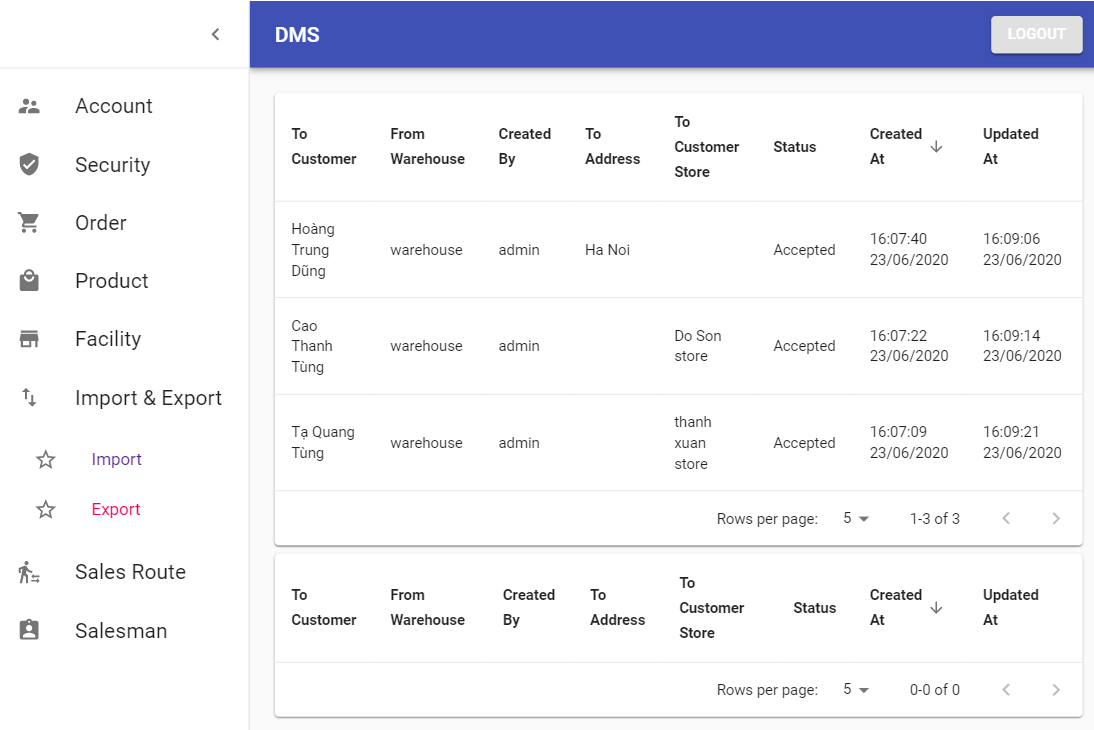
\includegraphics[width=15cm]{images/demo/view-export.png}
\caption{Quản lý xuất kho}
\end{figure}

% Chức năng thêm mới cửa hàng bán lẻ, hỗ trợ bản đồ
% Google Map để xác định vị trí.
% \begin{figure}[H]
% \centering
% 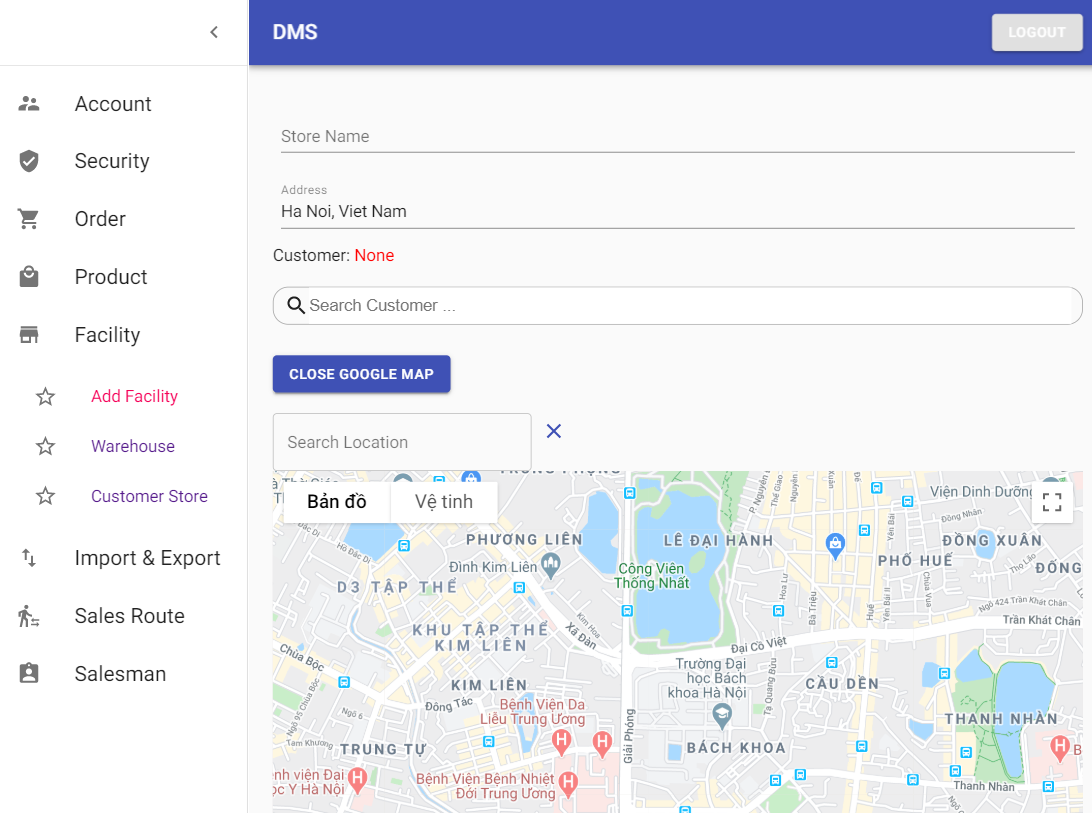
\includegraphics[width=15cm]{images/demo/add-customer-store.png}
% \caption{Thêm mới một cửa hàng bán lẻ}
% \end{figure}

% Chức năng tạo lịch trình tuyến bán hàng, sử dụng thuật toán
% K-Means phân cụm các cửa hàng bán lẻ, từ đó người quản lý
% chọn ra tuyến bán hàng phù hợp nhất cho nhân viên bán hàng.
% \begin{figure}[H]
% \centering
% 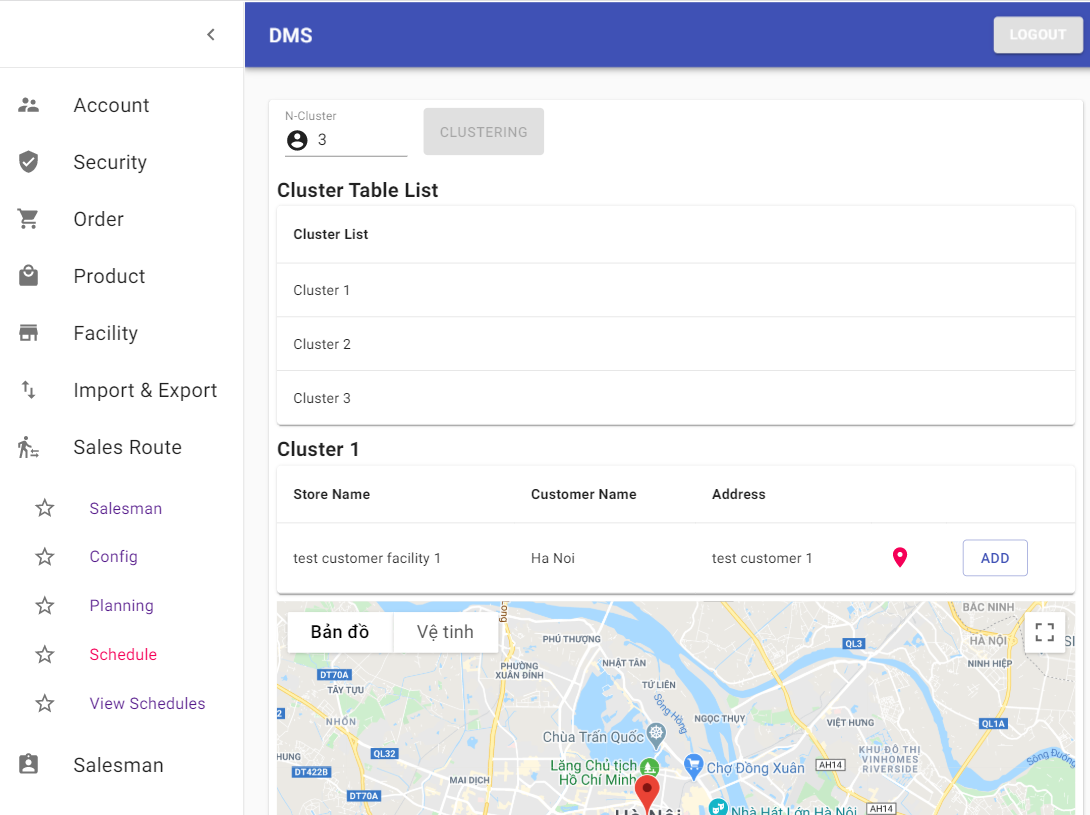
\includegraphics[width=15cm]{images/demo/add-schedule.png}
% \caption{Tạo lịch trình tuyến bán hàng}
% \end{figure}

% \begin{figure}[H]
% \centering
% 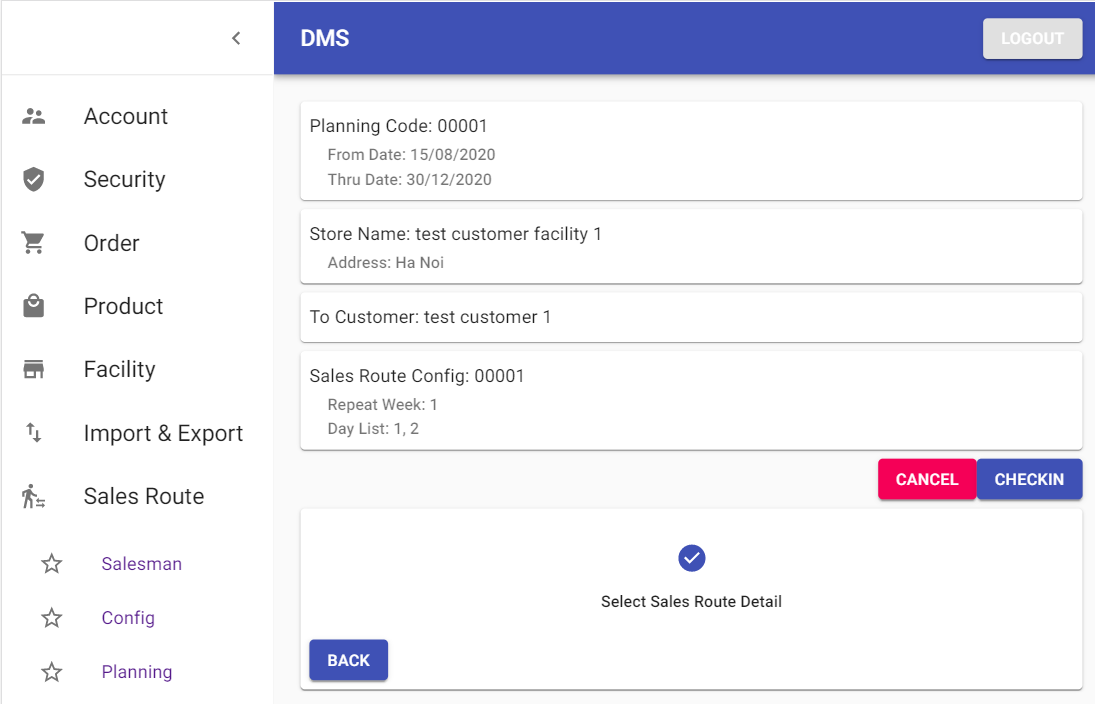
\includegraphics[width=15cm]{images/demo/salesman-checkin.png}
% \caption{Salesman check-in}
% \end{figure}
